\newcommand{\templatesdir}{../../../templates}
\newcommand{\template}{template-roteiro-est}
\input{\templatesdir/\template/template}

\newcommand{\content}{Listas dinâmicas}
\newcommand{\class}{Algoritmos e Estruturas de Dados}
\newcommand{\shortcourse}{45EST}

\begin{document}

\makeheader

{
Leitura obrigatória:
\begin{itemize}
	\item Capítulo 7 de~\cite{GoodrichEtAl2014} -- Listas e iteradores.
\end{itemize}

Leitura complementar:
\begin{itemize}
	\item Capítulo 5 de~\cite{Lafore2004} -- Listas encadeadas.
	\item Capítulo 7 de~\cite{Pereira2008} -- Listas encadeadas.
\end{itemize}
}

\medskip

\newtitle{Listas}

Pilhas, filas e deques:
\begin{itemize}
	\item Eficientes. \inblock{$\gets$ operações $O(1)$.}
	\item Permitem inserção/remoção nas extremidades.
\end{itemize}

\textbf{Lista dinâmica:} estrutura que permite operações em posições arbitrárias.

\medskip

Principais métodos:
\begin{itemize}
	\item \texttt{get(i)}: retorna o $i$-ésimo elemento da lista.
	\item \texttt{set(i,\,e)}: substitui o $i$-ésimo elemento por $e$.
	\item \texttt{add(i,\,e)}: adiciona $e$ na posição $i$ e desloca os demais elementos.
	\item \texttt{remove(i)}: remove o $i$-ésimo elemento da lista.
\end{itemize}

\clearpage

Exemplo de funcionamento:

\begin{figure}[H]
	\centering
	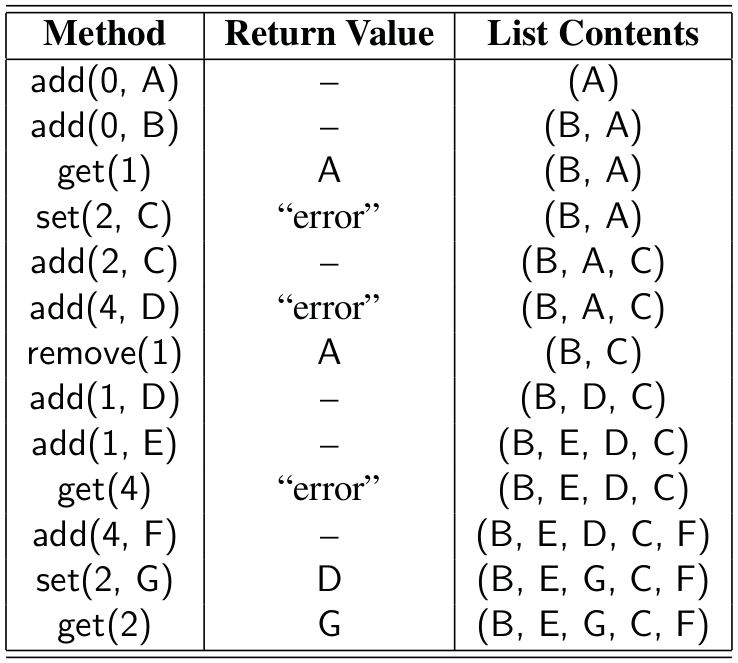
\includegraphics[width=0.5\linewidth]{img/table-7-1}
\end{figure}

Interface \texttt{List}:
\begin{minted}{java}
public interface List<E> {
	int size();
	boolean isEmpty();
	E get(int i);
	E set(int i, E e);
	void add(int i, E e);
	E remove(int i);
}
\end{minted}

\medskip


Implementação com vetores:
\begin{itemize}
	\item Elementos precisam ser realocados.
	\item Tamanho estático da estrutura.
\end{itemize}

Implementação com encadeamento:
\begin{itemize}
	\item Operação interna implica em percorrer a lista.
\end{itemize}

Realocação dos elementos de um vetor:

\begin{itemize}
	\color{redtext}
	\item Na inserção, todos os elementos são movidos para trás.
\end{itemize}

\begin{figure}[H]
	\centering
	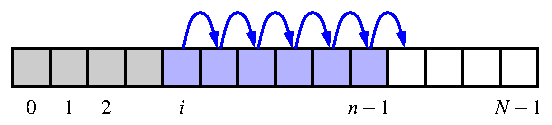
\includegraphics[width=0.7\linewidth]{img/figure-7-1a}
\end{figure}

\begin{itemize}
	\color{redtext}
	\item Na remoção, todos os elementos são movidos para frente.
\end{itemize}

\begin{figure}[H]
	\centering
	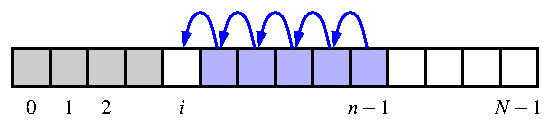
\includegraphics[width=0.7\linewidth]{img/figure-7-1b}
\end{figure}

Contornando a estrutura fixa de um vetor:
\begin{itemize}
	\item Mantém uma lista de tamanho fixo.
	\item Quando precisar de mais espaço, dobra o tamanho da lista.
	\begin{itemize}
		\item Cria uma nova (maior) lista.
		\item Copia os elementos para a nova lista.
		\item Atualiza a referência.
	\end{itemize}
\end{itemize}

\begin{figure}[H]
	\centering
	\begin{subfigure}
		\centering
		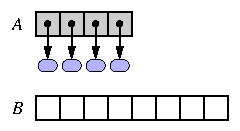
\includegraphics[width=0.32\linewidth]{img/figure-7-3a}
	\end{subfigure}%
	\begin{subfigure}
		\centering
		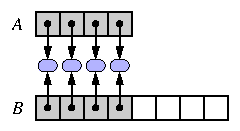
\includegraphics[width=0.32\linewidth]{img/figure-7-3b}
	\end{subfigure}%
	\begin{subfigure}
		\centering
		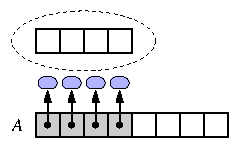
\includegraphics[width=0.32\linewidth]{img/figure-7-3c}
	\end{subfigure}
\end{figure}

\clearpage

Implementação baseada em vetores:
\begin{minted}{java}
public class ArrayList<E> implements List<E> {
	public static final int CAPACITY=16;
	private E[] data;
	private int size = 0;
	
	public ArrayList() { this(CAPACITY); }
	
	public ArrayList(int capacity) {
		data = (E[]) new Object[capacity];
	}
	
	public int size() { return size; }
	public boolean isEmpty() { return size == 0; }
	
	public E get(int i) {
		checkIndex(i, size);
		return data[i];
	}
	
	public E set(int i, E e) {
		checkIndex(i, size);
		E temp = data[i];
		data[i] = e;
		return temp;
	}
	
	public void add(int i, E e) {
		checkIndex(i, size + 1);
		if (size == data.length)
			resize(2 * data.length);
		for (int k=size-1; k >= i; k--)
			data[k+1] = data[k];
		data[i] = e;
		size++;
	}
	
	public E remove(int i) {
		checkIndex(i, size);
		E temp = data[i];
		for (int k=i; k < size-1; k++)
			data[k] = data[k+1];
		data[size-1] = null;
		size--;
		return temp;
	}
	
	protected void checkIndex(int i, int n) {
		if (i < 0 || i >= n)
			throw new IndexOutOfBoundsException("Illegal index: " + i);
	}
	
	protected void resize(int capacity) {
		E[] temp = (E[]) new Object[capacity];
		for (int k=0; k < size; k++)
			temp[k] = data[k];
		data = temp;
	}
	
	public String toString() {
		StringBuilder sb = new StringBuilder("(");
		for (int j = 0; j < size; j++) {
			if (j > 0) sb.append(", ");
			sb.append(data[j]);
		}
		sb.append(")");
		return sb.toString();
	}
}	
\end{minted}

\medskip

{\color{redtext}Comentários:}
\begin{itemize}
	\color{redtext}
	\item O método \texttt{checkIndex} verifica se não será acessada uma posição fora da lista.
	\item Na adição, caso se atinja o limite de tamanho do vetor, é chamado o método \texttt{resize} para aumentar sua capacidade e, então, inserir o elemento.
	\item A adição implica em movimentar todos os elementos seguintes.
	\item A remoção implica em movimentar todos os elementos seguintes.
\end{itemize}

\medskip

\textbf{Implementação baseada em listas encadeadas}

\medskip

Criação de métodos de acesso aleatório na lista duplamente encadeada:
\begin{minted}{java}
public class DoublyLinkedList<E> {
	
	/* ...
	* Complete implementation
	*/
	
	public void add(int position, E e) {
		checkIndex(position, size + 1);
		Node<E> n = searchNode(position);
		addBetween(e, n.getPrev(), n);
	}
	
	public E get(int position) {
		checkIndex(position, size);
		return(searchNode(position).getElement());
	}
	
	public E set(int position, E e) {
		checkIndex(position, size);
		Node<E> n = searchNode(position);
		addBetween(e, n, n.getNext());
		remove(n);
		return n.getElement();
	}
	
	public E remove(int position) {
		checkIndex(position, size);
		return remove(searchNode(position));
	}
	
	protected Node<E> searchNode(int position) {
		if(position == 0) return header.getNext();
		if(position == size()) return trailer;
		
		int count = -1;
		Node<E> walk = header.getNext();
		while(walk != trailer) {
			count++;
			if(count == position) {
				return walk;
			}
			walk = walk.getNext();
		}
		return null;
	}
	
	protected void checkIndex(int i, int n) {
		if (i < 0 || i >= n)
			throw new IndexOutOfBoundsException("Illegal index: " + i);
	}
}
\end{minted}

\medskip

{\color{redtext}Comentários:}
\begin{itemize}
	\color{redtext}
	\item Antes de cada operação é verificada a posição de acesso.
	\item O método \texttt{searchNode} recupera o nodo da posição $i$.
	\item Os métodos básicos são usados após encontrar a posição.
\end{itemize}

\medskip

Implementação da classe \texttt{LinkedList}:
\begin{minted}{java}
public class LinkedList<E> implements List<E> {
	DoublyLinkedList<E> list = new DoublyLinkedList<>();
	public int size() { return list.size(); }
	public boolean isEmpty() { return list.isEmpty(); }
	public String toString() { return list.toString(); }
	public E get(int i) { return list.get(i); }
	public E set(int i, E e) { return list.set(i, e); }
	public void add(int i, E e) { list.add(i, e); }
	public E remove(int i) { return list.remove(i); }
}
\end{minted}

\medskip

Comparação de complexidade:

\begin{table}[H]
	\centering
	\begin{tabular}{lll}
		\hline
		Operação & \texttt{ArrayList} & \texttt{LinkedList} \\
		\hline
		\texttt{get(i)} & $O(1)$ & $O(n)$ \\
		\texttt{set(i,\,e)} & $O(1)$ & $O(n)$\\
		\texttt{add(i,\,e)} & $O(n)$& $O(n)$\\
		\texttt{remove(i)} & $O(n)$ &$O(n)$ \\
		\hline
	\end{tabular}
\end{table}

\medskip

\underline{Exercícios:}
\begin{enumerate}
	\item Implemente listas dinâmicas baseadas em vetores e encadeamento para armazenar dados de filmes de uma locadora (título, gênero e ano). Implemente operações de inserção, remoção, consulta e listagem de filmes.
\end{enumerate}

\clearpage

\newtitle{Listas posicionais}

Ideia geral:
\begin{itemize}
	\item Resolver a ineficiência da \texttt{LinkedList}.
	\item Outras formas para determinar a posição de um elemento:
	\begin{itemize}
		\item Acessar diretamente os nodos $\to$ perde-se encapsulamento.
		\item Fornecer uma interface para acesso aos nodos $\to$ posições.
	\end{itemize}
	\item A posição de um elemento nunca muda, diferente do uso de índices.
	\item Exemplo: editor de texto (caracteres e cursor).
\end{itemize}

\medskip

Interface \texttt{Position}:
\begin{minted}{java}
public interface Position<E> {
	E getElement();
}
\end{minted}

\bigskip

TAD lista posicional:
\begin{itemize}
	\item Métodos de acesso em função de uma posição:
	\begin{itemize}
		\item \texttt{first()}/\texttt{last()} retornam a \textbf{posição} dos elementos.
		\item \texttt{before(p)}/\texttt{after(p)} retornam \textbf{posições} antes/depois de outra.
		\item {\color{redtext}Para acessar o elemento $\to$ \texttt{first().getElement()}.}
	\end{itemize}
	\item Métodos de atualização:
	\begin{itemize}
		\item \texttt{addFirst(e)}/\texttt{addLast(e)}
		\item \texttt{addBefore(p,\,e)}/\texttt{addAfter(p,\,e)}
		\item \texttt{set(p,\,e)}/\texttt{remove(p)}.
	\end{itemize}
\end{itemize}

\medskip

Exemplo de funcionamento:

\begin{figure}[H]
	\centering
	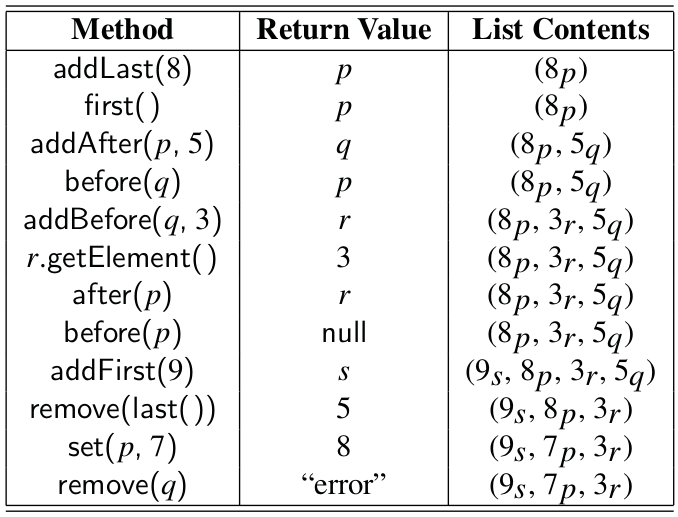
\includegraphics[width=0.55\linewidth]{img/table-7-4}
\end{figure}

Interface \texttt{PositionalList}:
\begin{minted}{java}
public interface PositionalList<E> {
	int size();
	boolean isEmpty();
	Position<E> first();
	Position<E> last();
	Position<E> before(Position<E> p);
	Position<E> after(Position<E> p);
	Position<E> addFirst(E e);
	Position<E> addLast(E e);
	Position<E> addBefore(Position<E> p, E e);
	Position<E> addAfter(Position<E> p, E e);
	E set(Position<E> p, E e);
	E remove(Position<E> p);
}
\end{minted}

\clearpage

Implementação baseada em encadeadamento:
\begin{minted}{java}
public class LinkedPositionalList<E> implements PositionalList<E> {
	
	private static class Node<E> implements Position<E> {
		private E element;
		private Node<E> prev;
		private Node<E> next;
		
		public Node(E e, Node<E> p, Node<E> n) {
			element = e;
			prev = p;
			next = n;
		}
		
		public E getElement() {
			if (next == null)
				throw new IllegalStateException("Pos. no longer valid");
			return element;
		}
		
		public Node<E> getPrev() {
			return prev;
		}
		
		public Node<E> getNext() {
			return next;
		}
		
		public void setElement(E e) {
			element = e;
		}
		
		public void setPrev(Node<E> p) {
			prev = p;
		}
		
		public void setNext(Node<E> n) {
			next = n;
		}
	}
	
	private Node<E> header;
	private Node<E> trailer;
	private int size = 0;
	
	public LinkedPositionalList() {
		header = new Node<>(null, null, null);
		trailer = new Node<>(null, header, null);
		header.setNext(trailer);
	}
	
	private Node<E> validate(Position<E> p) {
		if (!(p instanceof Node))
			throw new IllegalArgumentException("Invalid p");
		Node<E> node = (Node<E>) p;
		if (node.getNext() == null)
			throw new IllegalArgumentException("p is not in the list");
		return node;
	}
	
	private Position<E> position(Node<E> node) {
		if (node == header || node == trailer)
			return null;
		return node;
	}
	
	public int size() {
		return size;
	}
	
	public boolean isEmpty() {
		return size == 0;
	}
	
	public Position<E> first() {
		return position(header.getNext());
	}
	
	public Position<E> last() {
		return position(trailer.getPrev());
	}
	
	public Position<E> before(Position<E> p) {
		Node<E> node = validate(p);
		return position(node.getPrev());
	}
	
	public Position<E> after(Position<E> p) {
		Node<E> node = validate(p);
		return position(node.getNext());
	}
	
	private Position<E> addBetween(E e, Node<E> pred, Node<E> succ) {
		Node<E> newest = new Node<>(e, pred, succ);
		pred.setNext(newest);
		succ.setPrev(newest);
		size++;
		return newest;
	}
	
	public Position<E> addFirst(E e) {
		return addBetween(e, header, header.getNext());
	}
	
	public Position<E> addLast(E e) {
		return addBetween(e, trailer.getPrev(), trailer);
	}
	
	public Position<E> addBefore(Position<E> p, E e) {
		Node<E> node = validate(p);
		return addBetween(e, node.getPrev(), node);
	}
	
	public Position<E> addAfter(Position<E> p, E e) {
		Node<E> node = validate(p);
		return addBetween(e, node, node.getNext());
	}
	
	public E set(Position<E> p, E e) {
		Node<E> node = validate(p);
		E answer = node.getElement();
		node.setElement(e);
		return answer;
	}
	
	public E remove(Position<E> p) {
		Node<E> node = validate(p);
		Node<E> predecessor = node.getPrev();
		Node<E> successor = node.getNext();
		predecessor.setNext(successor);
		successor.setPrev(predecessor);
		size--;
		E answer = node.getElement();
		node.setElement(null);
		node.setNext(null);
		node.setPrev(null);
		return answer;
	}
		
	public String toString() {
		StringBuilder sb = new StringBuilder("(");
		Node<E> walk = header.getNext();
		while (walk != trailer) {
			sb.append(walk.getElement());
			walk = walk.getNext();
			if (walk != trailer)
			sb.append(", ");
		}
		sb.append(")");
		return sb.toString();
	}
}
\end{minted}

\medskip

{\color{redtext}
Comentários:
\begin{itemize}
	\item Implementação baseada em uma lista duplamente encadeada.
	\item Os nodos são as posições, mas o único aspecto visível externamente é o método \texttt{getElement}.
	\item Método \texttt{validate} faz a conversão de posição para nodo.
	\item Método \texttt{position} devolve o nodo convertido em posição.
	\item Uma posição inexistente é identificada pelos seus campos nulos.
\end{itemize}
}

\medskip

\textbf{OBS:} uma vez conhecida a posição, todas as operações de uma lista posicional executam em tempo constante $O(1)$.

\medskip

\newtitle{Atividades}

\begin{enumerate}
	\item Modifique o código das classes \texttt{ArrayList} e \texttt{LinkedList} e implemente um método \texttt{add(e)} que insere o elemento $e$ no final da lista.
	
	\item A complexidade dos métodos utilizados pela \texttt{LinkedList} origina-se no procedimento \texttt{searchNode}, reponsável por buscar o nodo da posição que se deseja acessar. O desempenho dessa estrutura de dados pode ser melhorado inibindo essa busca quando tratar-se de acesso ao início ou fim da lista. Implemente essa estratégia.
	
	\item Outra forma de melhorar o desempenho de uma \texttt{LinkedList} é fazer com que a busca implementada no procedimento \texttt{searchNode} seja feita de ``trás para frente'', quando conveniente. Implemente essa estratégia. Qual o impacto na complexidade prática do procedimento de busca?
	
	\item Crie um método \texttt{toArray} na classe \texttt{LinkedList} que retorne um vetor com os elementos da lista encadeada. Implemente a operação inversa na classe \texttt{ArrayList}.
	
	\item Como seria uma lista posicional implementada baseada em vetores (\texttt{ArrayPositionalList})? Manter apenas o índice onde o elemento está armazenado é suficiente para mapear sua posição? Implemente essa estrutura de dados.
	
	\item Leia a respeito do uso de iteradores para percorrer uma lista e acessar seus elementos~\citep{GoodrichEtAl2014}.
	
	\bigskip
	
	\item Resolva os seguintes exercícios de~\cite{GoodrichEtAl2014}:
	\begin{itemize}
		\item[R-7.1:] Projete uma representação de uma lista \texttt{L} inicialmente vazia após realizar as seguintes operações: \texttt{add(0,\,4)}, \texttt{add(0,\,3)}, \texttt{add(0,\,2)}, \texttt{add(2,\,1)}, \texttt{add(1,\,5)}, \texttt{add(1,\,6)}, \texttt{add(3,\,7)}, \texttt{add(0,\,8)}.
		
		\item[R-7.2:] Implemente uma pilha usando um \texttt{ArrayList} para armazenamento.
		
		\item[R-7.3:] Implemente um deque usando um \texttt{ArrayList} para armazenamento.
		
		\item[R-7.5:] O \texttt{java.util.ArrayList} possui um método \texttt{trimToSize} que substitui o vetor correspondente por um com capacidade equivalente ao número de elementos atuais da lista. Implemente tal método para a verão dinâmica da classe \texttt{ArrayList}.
		
		\item[R-7.7:] Considere uma implementação de um \texttt{ArrayList} usando um vetor dinâmico, mas ao invés de copiar os elementos para um vetor com o dobro do tamanho (isto é, de $N$ para $2N$) quando sua capacidade é atingida, copiamos os elementos para um vetor com $\lceil N/4 \rceil$ células adicionais, indo da capacidade $N$ para $N + \lceil N/4 \rceil$. Mostre que ao realizar uma sequência de $n$ operações \texttt{push} (isto é, inserindo no fim) ainda opera em tempo $O(n)$. 
		
		\item[R-7.8:] Supondo que estamos mantendo uma coleção \texttt{C} de elementos de tal modo que, cada vez que adicionamos um novo elemento na coleção, copiamos o conteúdo de \texttt{C} em um novo \texttt{ArrayList} do tamanho exato ao necessário. Qual é o tempo de processamento de adição de $n$ elementos em uma coleção \texttt{C} inicialmente vazia?
		
		\item[R-7.9:] O método \texttt{add} para um vetor dinâmico tem a seguinte ineficiência: no caso em que um redimensionamento ocorre, a operação correspondente leva tempo para copiar todos os elementos do antigo vetor para o novo, e então o laço subsequente muda alguns deles para dar espaço para o novo elemento. Modifique o método \texttt{add} para, no caso de redimensionamento, os elementos copiados ficarem na sua posição final do novo vetor (ou seja, nenhuma realocação deve ser feita).
		
		\item[R-7.10:] Reimplemente a classe \texttt{ArrayStack} usando vetores dinâmicos para suportar uma capacidade ilimitada.
		
		\item[R-7.12:] Supondo que queremos estender nossa \texttt{PositionalList} com um método \texttt{indexOf(p)}, que retorna o índice atual do elemento armazenado na posição \texttt{p}. Mostre como implementar esse método usando apenas outros métodos da interface \texttt{PositionalList} (sem detalhes da nossa implementação \texttt{LinkedPositionalList}).
		
		\item[R-7.13:] Supondo que queremos estender nossa \texttt{PositionalList} com um método \texttt{findPosition(e)}, que retorna a primeira posição contendo um elemento igual a \texttt{e} (ou \texttt{null} se tal posição não existir). Mostre como implementar esse método usando apenas métodos existente da interface \texttt{PositionalList} (sem detalhes da nossa implementação \texttt{LinkedPositionalList}).
		
		\item[R-7.14:] A implementação \texttt{LinkedPositionalList} não realiza nenhuma verificação de erro para testar se uma posição \texttt{p} dada é um membro relevante da lista. Explique detalhadamente o efeito da chamada \texttt{L.addAfter(p,\,e)} de uma lista \texttt{L} com uma posição \texttt{p} que pertence a alguma outra lista \texttt{M}.
		
		\item[R-7.15:] Para melhor modelar uma fila (FIFO) cujas entradas possam ser deletadas antes de chegar à frente da mesma, projete uma classe \texttt{LinkedPositionalQueue} que suporte o tipo abstrato fila, com o método \texttt{enqueue} retornando uma instância de posição e suporte um novo método \texttt{remove(p)}, que remove e retorna o elemento associado com a posição \texttt{p} da fila. Você pode usar uma \texttt{LinkedPositionalList} para armazenamento.
		
		\item[R-7.18:] A interface \texttt{java.util.Collection} inclui um método \texttt{contains(o)}, que retorna \texttt{true} se a coleção possui um objeto que é igual a \texttt{Object o}. Implemente tal método na classe \texttt{ArrayList}.
		
		\item[R-7.19:] A interface \texttt{java.util.Collection} inclui um método \texttt{clear()}, que remove todos os elementos de uma coleção. Implemente tal método na classe \texttt{ArrayList}.
		
		\item[C-7.25:] Implemente uma lista baseada em vetores com capacidade fixa e tratamento circular, que chegue a um tempo $O(1)$ para inserções e remoções no índice 0, bem como para inserções e remoções no final da lista. Sua implementação também deverá fornecer um método \texttt{get} de tempo constante.
		
		\item[C-7.26:] Complete o exercício anterior, mas usando um vetor dinâmico com capacidade ilimitada.
		
		\item[C-7.35:] Reimplemente a classe \texttt{ArrayQueue} usando um vetor dinâmico para suportar capacidade ilimitada. Seja cuidadoso no tratamento circular do vetor no momento do redimensionamento.
		
		\item[P-7.58:] Desenvolva um experimento para testar a eficiência de $n$ chamadas sucessivas ao método \texttt{add} de um \texttt{ArrayList} para vários $n$ diferentes, sob cada um dos seguintes cenários:
		\begin{enumerate}[a.]
			\item Cada \texttt{add} acontece no índice $0$.
			\item Cada \texttt{add} acontece no índice \texttt{size()/2}.
			\item Cada \texttt{add} acontece no índice \texttt{size()}.
			\item Analise seus resultados empíricos.
		\end{enumerate}
		
		\item[P-7.60:] Implemente uma classe \texttt{CardHand} que suporta uma pessoa ordenando um grupo de cartas na sua mão. O simulador deverá representar uma sequência de cartas utilizando uma lista posicional única, de tal modo que cartas do mesmo naipe são mantidas juntas. Implemente esta estrategia considerando quatro ``dedos'', cada um armazenando cartas de um dos naipes (copas, paus, espadas e ouros). Assim, adicionar uma nova carta na mão da pessoa ou jogar uma carta da mão pode ser feito em tempo constante. A classe deve suportar os seguintes métodos:
		\begin{itemize}
			\item \texttt{addCard(r,\,s)}: adiciona uma nova carta com número \texttt{r} e naipe \texttt{s} para a mão.
			\item \texttt{play(s)}: remove e retorna uma carta de naipe \texttt{s} da mão do jogador. Se não existir carta do naipe \texttt{s}, então remove e retorne uma carta arbitrária da mão.
		\end{itemize}
	\end{itemize}
\end{enumerate}

\medskip

\newtitle{Referências}
\begingroup
	\footnotesize
	\renewcommand{\chapter}[2]{}%
	\bibliographystyle{apalike}
	\bibliography{../referencias}
\endgroup

\end{document}